\chapter{ニューラルネットワークの学習について}

\section{学習の様子}
	評価実験で用いたBERT+weight, BERT, embeddingの3手法について,
	それぞれのネットワーク学習時のふるまいを示す.
	以下の図\ref{fig:BERT_plus_weight_loss}~\ref{fig:embedding_loss}は,
	各モデルを学習しているときの
	train loss, validation lossの推移を示したグラフである.

	\begin{figure}[H]
		\centering
		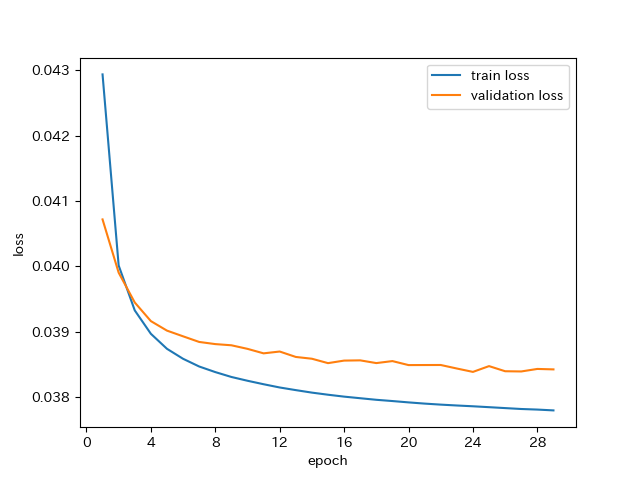
\includegraphics[keepaspectratio, scale=0.8]{./figure/BERT+weight.png}
		\caption{BERT+weightの学習中の各種lossの推移}
		\label{fig:BERT_plus_weight_loss}
	\end{figure}

	\begin{figure}[H]
		\centering
		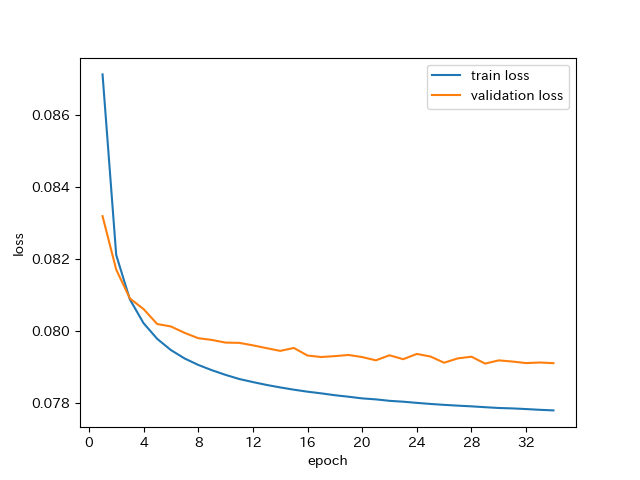
\includegraphics[keepaspectratio, scale=0.8]{./figure/BERT.png}
		\caption{BERTの学習中の各種lossの推移}
		\label{fig:BERT_loss}
	\end{figure}

	\begin{figure}[H]
		\centering
		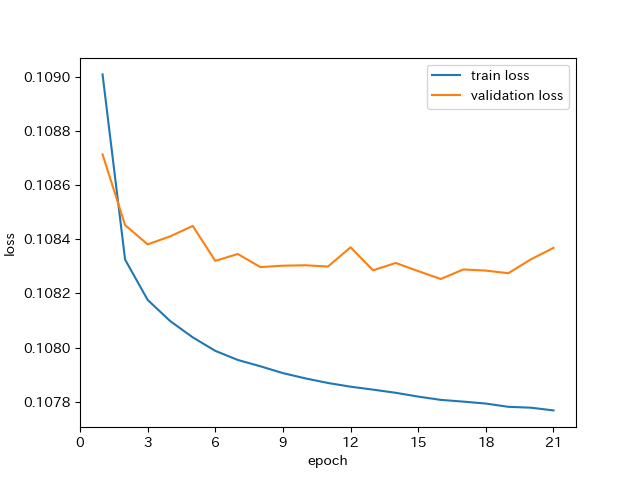
\includegraphics[keepaspectratio, scale=0.8]{./figure/embeddings.png}
		\caption{embeddingの学習中の各種lossの推移}
		\label{fig:embedding_loss}
	\end{figure}

	なお,学習についてはEarly Stoppingを採用している.
	5回以上validation lossが更新されなかった場合に学習を停止し,
	それ以前でvalidation lossが最良であったネットワークを用いた.
	この時,各ネットワークの学習に要したエポック数と
	その時のtest lossは以下の表\ref{table:epoch_num}の通りである.

	\begin{table}[H]
		\centering
		\caption{各手法におけるネットワーク学習に要したエポック数とtest loss}
		\label{table:epoch_num}
		\begin{tabular}{|c|c|c|}
			\hline
			& エポック数 & test loss \\
			\hline
			BERT+weight & 23 & 0.0384 \\
			\hline
			BERT & 28 & 0.0792 \\
			\hline
			embedding & 15 & 0.1082 \\
			\hline
		\end{tabular}
	\end{table}

\section{ウィンドウサイズによる性能の変化}
	データセット生成時に感性語の周辺単語を収集する範囲である
	ウィンドウサイズを変化させたときの
	性能の変化について,BERT+weightとBERTのそれぞれで検証した.
	以下の表\ref{table:window_size}にその結果を示す.

	\begin{table}[H]
		\centering
		\caption{ウィンドウサイズの変化によるtest lossの変化}
		\label{table:window_size}
		\begin{tabular}{|c|c|c|}
			\hline
			& $W=2$ & $W=3$ & $W=4$ \\
			\hline
			BERT+weight & 0.0294 & 0.0384 & 0.0446 \\
			BERT & 0.0670 & 0.0792 & 0.0863 \\